\documentclass{article}
\usepackage{listings}
\usepackage{xcolor}
\usepackage[margin=1in]{geometry}
\usepackage{graphicx}

\title{Lab 4}
\author{Nicholas Storti}

\begin{document}
\maketitle

\section{Output}

\begin{verbatim}
Setting up the problem...0.001136 s
Image: 300 x 500
Mask: 5 x 5
Allocating device variables...0.160549 s
Copying data from host to device...0.011650 s
Launching kernel...0.000037 s
Copying data from device to host...0.000310 s
Verifying results...TEST PASSED


Setting up the problem...0.004035 s
Image: 600 x 1000
Mask: 5 x 5
Allocating device variables...0.136232 s
Copying data from host to device...0.011440 s
Launching kernel...0.000042 s
Copying data from device to host...0.001178 s
Verifying results...TEST PASSED


Setting up the problem...0.014169 s
Image: 1080 x 1920
Mask: 5 x 5
Allocating device variables...0.136064 s
Copying data from host to device...0.011649 s
Launching kernel...0.000055 s
Copying data from device to host...0.001640 s
Verifying results...TEST PASSED


Setting up the problem...0.018313 s
Image: 1440 x 1920
Mask: 5 x 5
Allocating device variables...0.136463 s
Copying data from host to device...0.011787 s
Launching kernel...0.000065 s
Copying data from device to host...0.002126 s
Verifying results...TEST PASSED


Setting up the problem...0.054812 s
Image: 2160 x 3840
Mask: 5 x 5
Allocating device variables...0.137316 s
Copying data from host to device...0.012731 s
Launching kernel...0.000117 s
Copying data from device to host...0.004498 s
Verifying results...TEST PASSED


Setting up the problem...0.001923 s
Image: 500 x 500
Mask: 5 x 5
Allocating device variables...0.142000 s
Copying data from host to device...0.011336 s
Launching kernel...0.000038 s
Copying data from device to host...0.000495 s
Verifying results...TEST PASSED


Setting up the problem...0.007078 s
Image: 1000 x 1000
Mask: 5 x 5
Allocating device variables...0.136501 s
Copying data from host to device...0.011465 s
Launching kernel...0.000046 s
Copying data from device to host...0.001105 s
Verifying results...TEST PASSED


Setting up the problem...0.026603 s
Image: 2000 x 2000
Mask: 5 x 5
Allocating device variables...0.142042 s
Copying data from host to device...0.011999 s
Launching kernel...0.000076 s
Copying data from device to host...0.002336 s
Verifying results...TEST PASSED


Setting up the problem...0.059078 s
Image: 3000 x 3000
Mask: 5 x 5
Allocating device variables...0.136755 s
Copying data from host to device...0.012885 s
Launching kernel...0.000115 s
Copying data from device to host...0.005022 s
Verifying results...TEST PASSED


Setting up the problem...0.105080 s
Image: 4000 x 4000
Mask: 5 x 5
Allocating device variables...0.141408 s
Copying data from host to device...0.014098 s
Launching kernel...0.000192 s
Copying data from device to host...0.007331 s
Verifying results...TEST PASSED


Setting up the problem...0.164097 s
Image: 5000 x 5000
Mask: 5 x 5
Allocating device variables...0.142911 s
Copying data from host to device...0.015974 s
Launching kernel...0.000319 s
Copying data from device to host...0.011310 s
Verifying results...TEST PASSED


Setting up the problem...0.236086 s
Image: 6000 x 6000
Mask: 5 x 5
Allocating device variables...0.143743 s
Copying data from host to device...0.017801 s
Launching kernel...0.000451 s
Copying data from device to host...0.016059 s
Verifying results...TEST PASSED


Setting up the problem...0.321387 s
Image: 7000 x 7000
Mask: 5 x 5
Allocating device variables...0.137197 s
Copying data from host to device...0.019888 s
Launching kernel...0.000604 s
Copying data from device to host...0.022223 s
Verifying results...TEST PASSED


Setting up the problem...0.419108 s
Image: 8000 x 8000
Mask: 5 x 5
Allocating device variables...0.144746 s
Copying data from host to device...0.022349 s
Launching kernel...0.000783 s
Copying data from device to host...0.031572 s
Verifying results...TEST PASSED
\end{verbatim}

\section{Answer Section}

\begin{enumerate}
	\item What is the floating-point computation rate for the GPU kernel in this application? How does it scale with the size of the input image? To answer this question, try multiple sized inputs and calculate the rate for each using the timing measurements
	provided in the code. Make sure to justify your choice of input sizes. \\
	
	\begin{figure}[h]
		\centering
		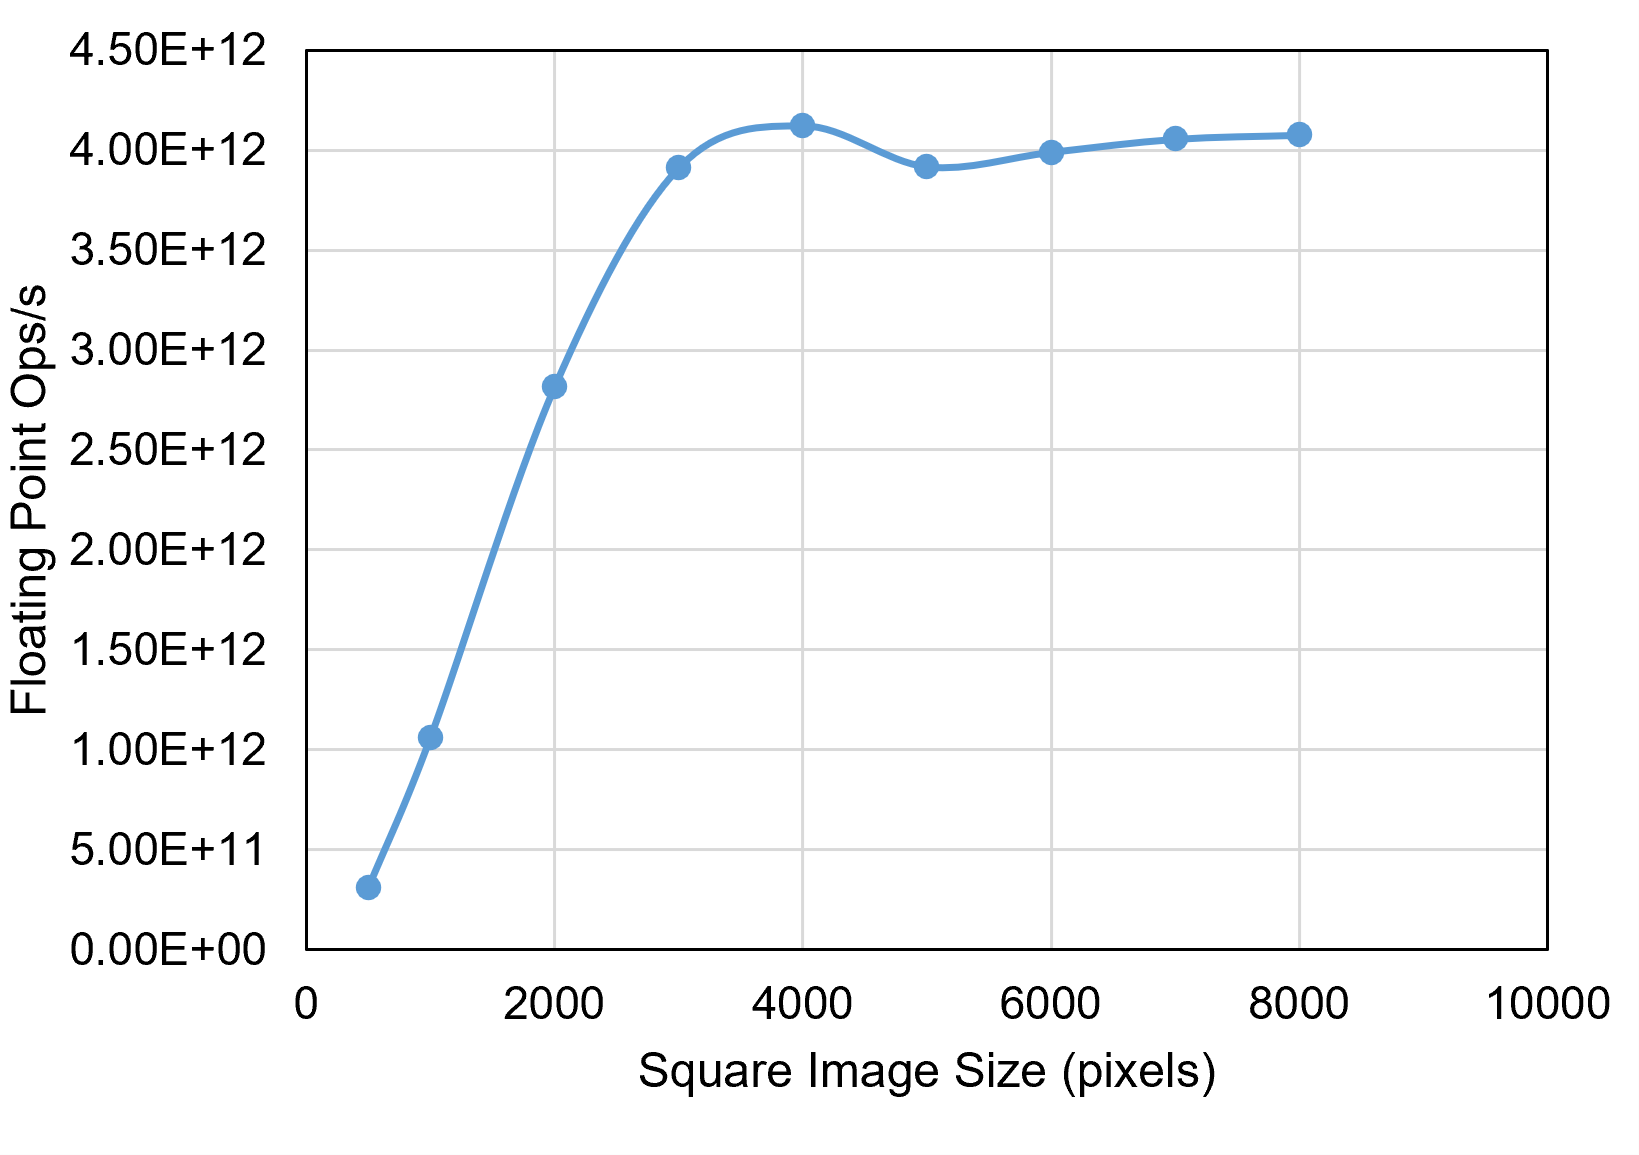
\includegraphics[width=0.75\linewidth]{FLOPS}
		\caption{Graph of FLOPS vs. input image size.}
	\end{figure}
	
	Below is a plot of the floating point computation rate in floating point operations per second (FLOPS) for the GPU kernel as a function of the size of the input image. Square input sizes were used so the comparison would be simple. Images can be found with resolution as low as 500x500 pixels, and some monitors can display images with a width up to 8000 pixels, so a range of image sizes between 500x500 and 8000x8000 were used. The filter size is 5x5, and for each filter element, a multiply and addition operation are performed. 2 floating point operations are thus performed for each filter element, and there are a total of 25 filter elements. The filter is applied to each pixel of the input image, so 50 floating point operations are performed for each pixel of the image. The total number of floating point operations is then $50 * (input\ image\ width) * (input\ image\ height)$. For square images, the number of operations is $50 * (image\ size)^2$. The FLOPS can then be calculated by dividing this total number of floating point operations by the kernel execution time provided in the output of the code. \\
	
	As the size of the input image increases, the FLOPS increase linearly until around 4000. After image size of 4000, the FLOPS level out around 4e12. So, for images below size 4000, the FLOPS scale linearly with input image size. For images larger than 4000x40000, the FLOPS stay constant.
	
	\item What percentage of time is spent as overhead for using the GPU? Consider as overhead: device memory allocation time and memory copy time to and from the device. Do not include problem setup time or result verification time in your calculations of overhead or total execution time. Try this with multiple input sizes and explain how the overhead scales with the size of your input? \\
	
	\begin{figure}[h]
		\centering
		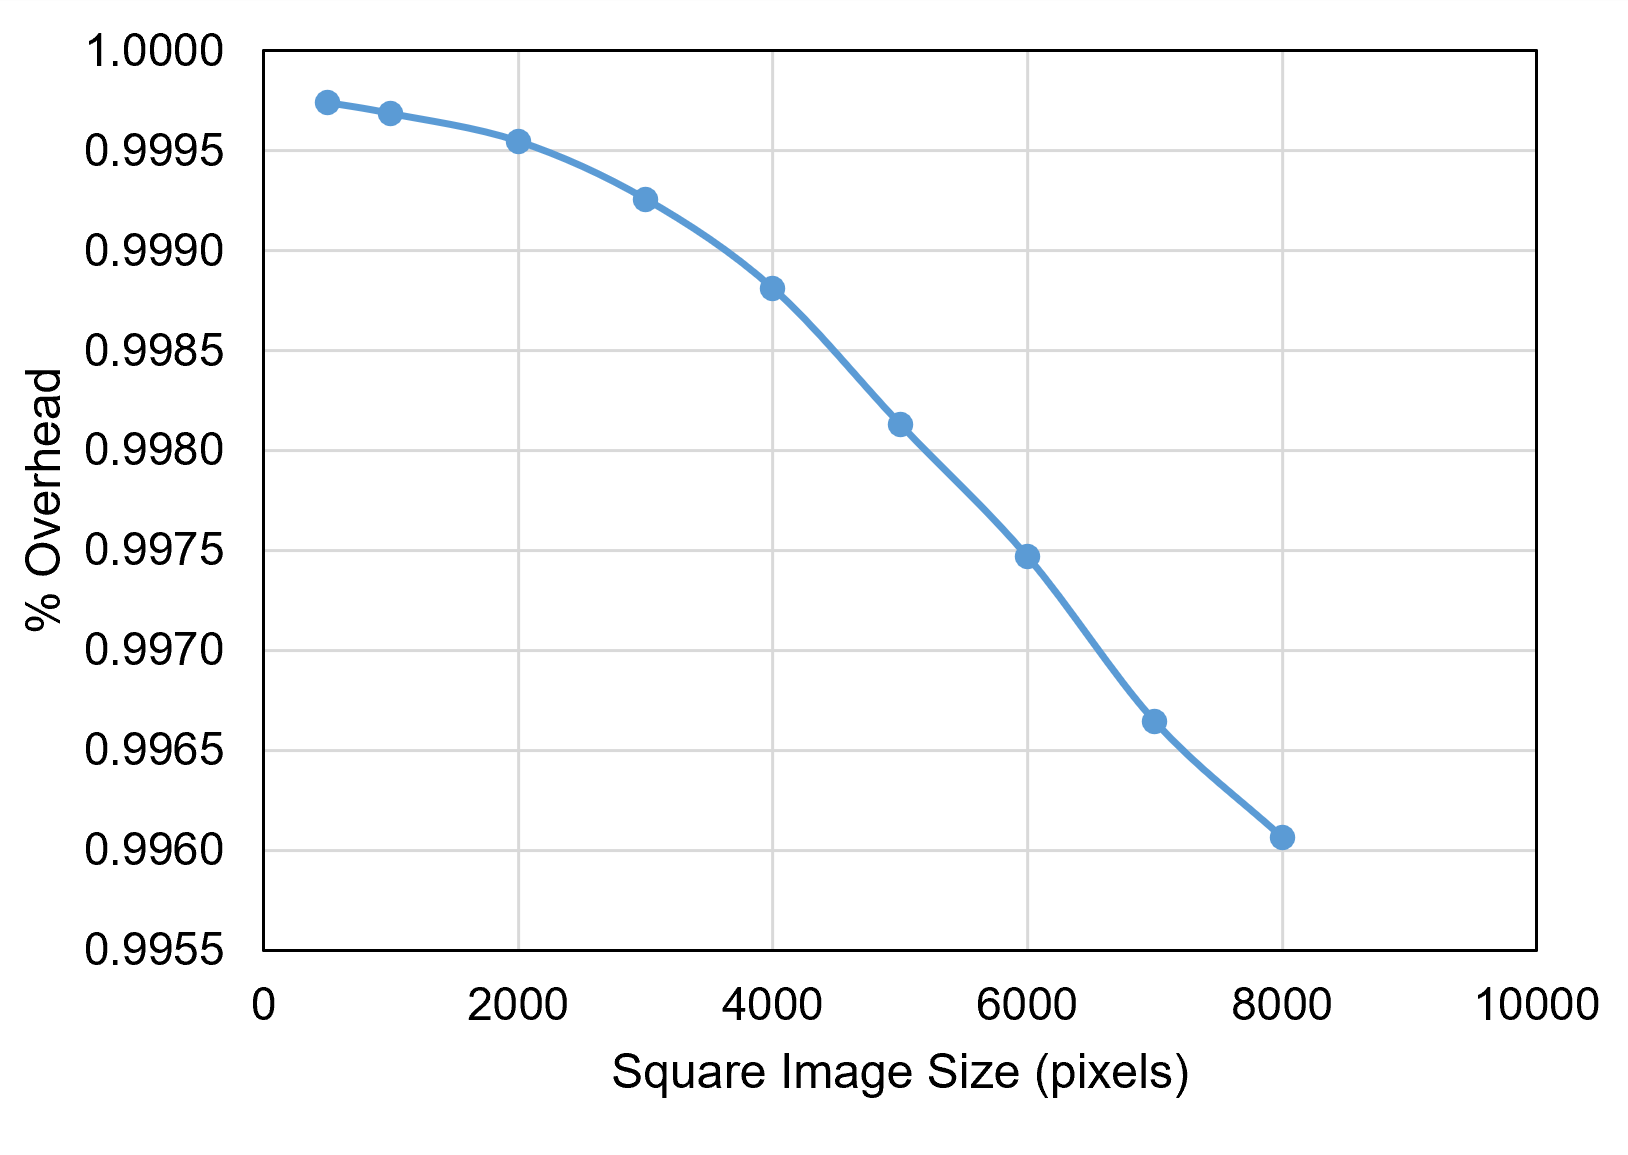
\includegraphics[width=0.75\linewidth]{Overhead}
		\caption{Percentage of time spent on overhead vs. input image size.}
	\end{figure}
	
	Shown below is a plot of percentage of time spent on overhead as a function of the size of the input image. Again, square input images with sizes in range 500x500 to 8000x8000 were used. Generally, for the input sizes tested, over 99\% of the time is spent on overhead for using the GPU. As the size of the input image increases, the percentage of time spent on overhead decreases. The time for allocation of device variables is constant in terms of input size. The time for copying data from host to device and vice versa increases linearly with the number of pixels in the input image. The kernel execution time also increases linearly with the number of pixels, but since the kernel performs multiple floating point operations, the kernel execution time increases linearly with a larger slope than the time for copying data. Because of this, the kernel execution time grows faster than the time for copying data as the image size increases. So, the percentage of time spent on kernel execution will increase with image size, and the percentage of time spent on overhead, specifically copying data, will decrease with image size. 
\end{enumerate}

\end{document}